\section{Object and Event selection}
\label{sec:AN_Selection}

In this chapter we document the electron, muon, and photon identification and isolation criteria, $E_T^{MET}$ criteria, and provide the results of comparing simulation with data.
%We use cut-based selection of lepton + photon + MET where lepton is either muon or electron. 
%Photon and MET selection are a little bit different for different channels. 
%The second lepton veto is applied.  dR(lep,pho)$>$0.7 where $dR=\sqrt{({d\phi}^2+{d\eta}^2)}$ 
%is applied to avoid divergence of ISR and FSR contributions. No restrictions applied on a number of
% photons in the event but the candidate with the hardest photon is selected in the particular event among 
%those photons which passed all the other cuts including dR. dR is also a part of the phase space selection.\\
%The plot of total data vs MC after the selection criteria applied is shown in Fig. \ref{fig:DATAvsMC}.

\subsection{Event Level Selection}

In the $W\gamma\rightarrow l\nu\gamma$ process we have a lepton, a photon, and a neutrino as final state particle. Therefore, we select events with exactly one lepton (muon or electron), a photon, both originating from the primary vertex, and with significant $E_T^{miss}$. The object selection criteria as well as criteria for the second lepton veto are desribed in Ch.~\ref{sec:AN_ObjectSelection}.

To select events with significant $E_T^{miss}$, we apply a cut on the transverse mass of a $W$~boson of $M_T^W>40$~GeV, where 
\begin{equation}
$M_T=\sqrt{(2 \cdot P_T^{Lep} \cdot P_T^{MET} \cdot (1-\cos{(\phi^{lep}-\phi^{MET})}))}$.
\end{equation}.

After that, there is still signifcant background from DY+jets$\rightarrow e e \gamma$ in the electron channel that originates from one of the electrons misidentified as a photon. This background is the most significant around the invariant mass of $e\gamma$ close to the mass of the $Z$ boson (Fig.~\ref{fig:DATAvsMC_Mpholep1}). To reject this background, we apply $Z$-mass window cut: events where $70$~GeV$<M_{e\gamma}<110$~GeV are rejected. 

Finally, the separation $\Delta R=\sqrt{({\Delta\phi}^2+{\Delta\eta}^2)}$ between the final state lepton and photon is required to be $\Delta R(l,\gamma)>0.7$ to avoid divergence coming from the ISR and FSR contributions and also to enchance the TGC contribution. In case if there are more than one photon in the event passed all selection criteria including the $\Delta R$ cut, the candidate with the hardest photon is selected (one with the highest $P_T^{\gamma}$). 

\begin{figure}[htb]
  \begin{center}
   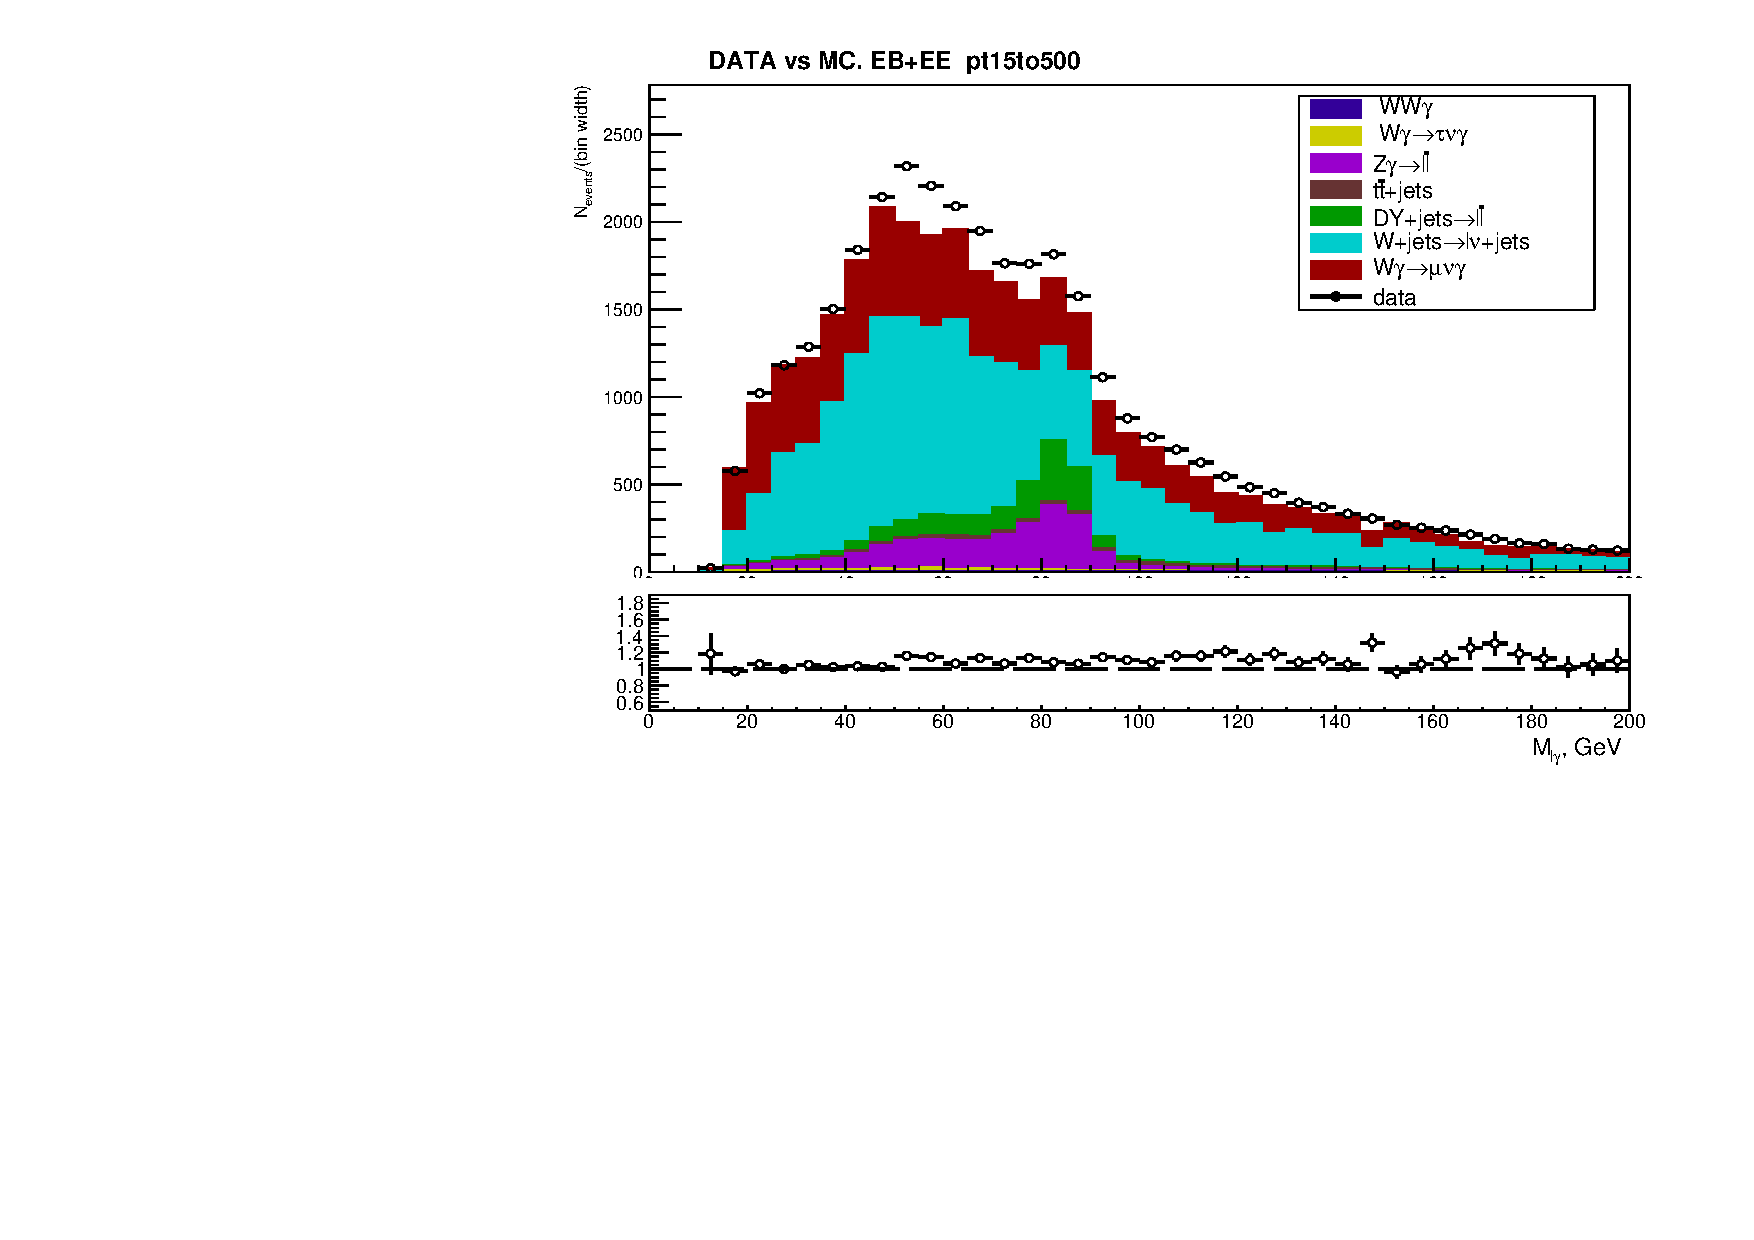
\includegraphics[width=0.5\textwidth]{../figs/figs_v11/MUON_WGamma/PrepareYields/c_TotalDATAvsMC_EtaCommon__Mpholep1_pt15to500_.pdf}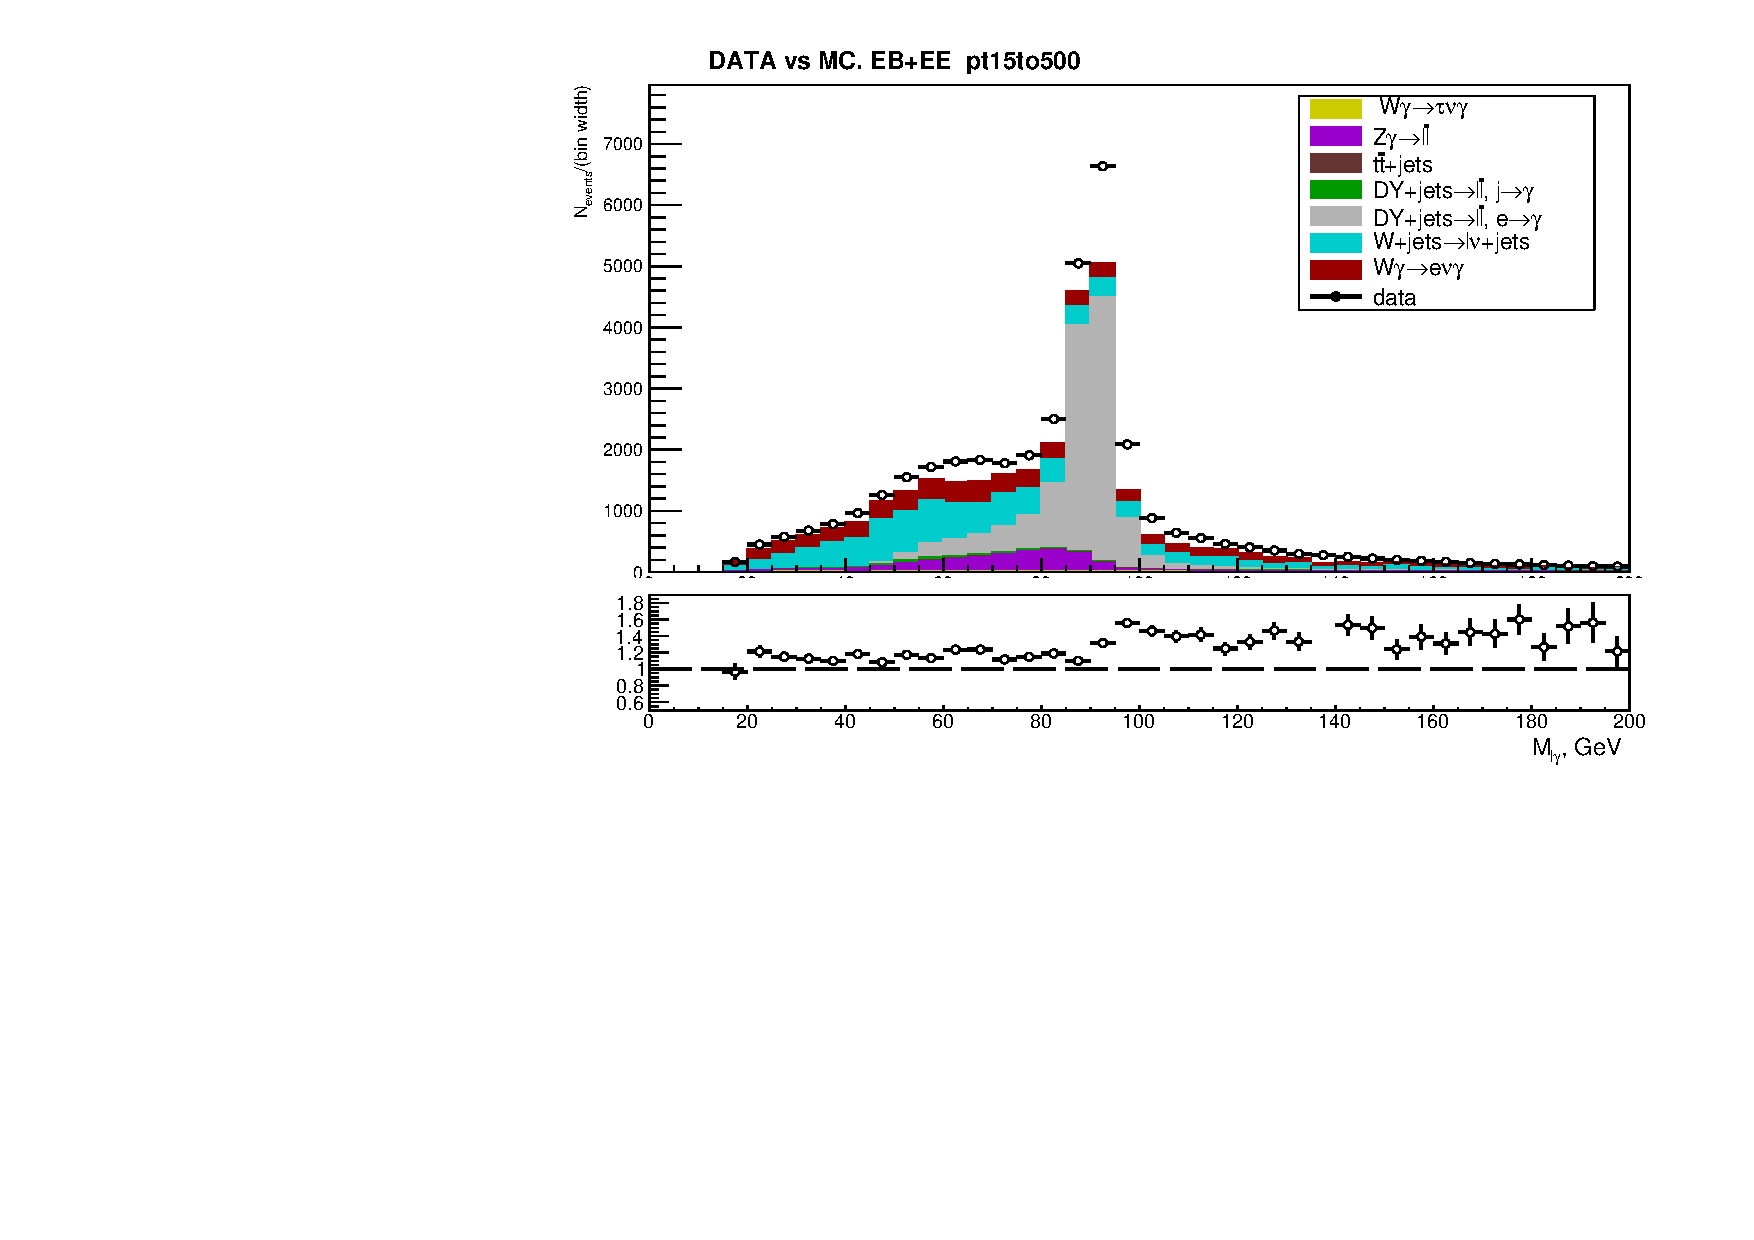
\includegraphics[width=0.5\textwidth]{../figs/figs_v11/ELECTRON_WGamma/PrepareYields/c_TotalDATAvsMC_EtaCommon__Mpholep1PRELIMINARY_FOR_E_TO_GAMMA_WITH_PSV_CUT_pt15to500_.pdf}
  \caption{Data vs MC plots, $M_{l,\gamma}$. Left - muon channel, right - electron. All selection criteria except $M_{l,\gamma}$ cut on these plots. $<P_T^{\gamma}>15$~GeV. The analysis cut of $M_{l,\gamma}<70~or~M_{l,\gamma}>110$~GeV is selected for the electron channel only.}
  \label{fig:DATAvsMC_Mpholep1}
  \end{center}
\end{figure}

\subsection{Object selection}
\label{sec:AN_ObjectSelection}

We select events with muons and photons in the final state for the muon channel and events with electrons and photons in the final state for the electron channel. CMS Particle Object Group (POG) all CMS physics measurements with their recommendation for object identification (ID) criteria for any given period of data-taking. For~2012 data recommendations included two sets of muon ID criteria: "Tight" and "Loose" and four sets of electron and photon ID criteria: "Tight", "Medium", "Loose" and "Veto".

For the muon selection, we applied the kinematics cuts of $p_T>25$ GeV and $|\eta|<2.1$ and "Tight" ID criteria. To reject events with two or more muons, like $Z\gamma\rightarrow\mu\mu\gamma$ events, we rejected all events that have the second reconstructed muon candidate with $P_T>10$ GeV and $|\eta|<2.4$. Data to MC scale factors are applied as recommended by CMS POG.

We consider electrons with $p_T>30$~GeV passing the "Tight" ID criteria and photons with $P_T>15$~GeV passing the modified "Medium" ID criteria. The modification of the photons ID criteria was studied in the $W\gamma\gamma \rightarrow l\nu\gamma\gamma$ measurement~\cite{ref_Wgg8TeV}. 

In addition, electrons and photons must be within the ECal acceptance that is defined in terms of barrel (EB) and endcap (EE) sections with pseudorapidity ranges of $|\eta| < 1.4442$ and $1.566 < |\eta| < 2.5$, respectively. To reject events with two or more final state electrons, events with the second reconstructed electron candidate with $p_T>10$ GeV and satisfying the "Veto" ID criteria are rejected. No restrictions on the maximum number of the final state photons is applied. 

Selection criteria are applied consistently on the data sample as well as on all MC samples. Due to various reasons, the selection efficiency may slightly differ between data and simulation. The efficiency ratios are called the scale factors. The scale factors for the selection criteria recommended by CMS POG are provided by CMS POG. For the modified photon ID criteria, the appropriate changes to the POG-recommended scale factors were applied derived by the $W\gamma\gamma$ team~\cite{ref_Wgg8TeV}.

% NEED PLOTS WITH SCALE FACTORS 

\subsection{Other details related to the event and object selection}

% ABOUT PILEUP

Weights are applied on each event in each simulation sample including weight due to pileup. The pile up reweighting is applied. Fig.~\ref{fig:DATAvsMC_nVtx} shows the distribution of the number of vertices for the $Z\gamma$ selected sample in muon channel before (left) and after (right) the pileup reweighting of the simulation samples. The same procedure of the pileup reweighting is applied for the $W\gamma$ selected simulation samples.

\begin{figure}[htb]
  \begin{center}
   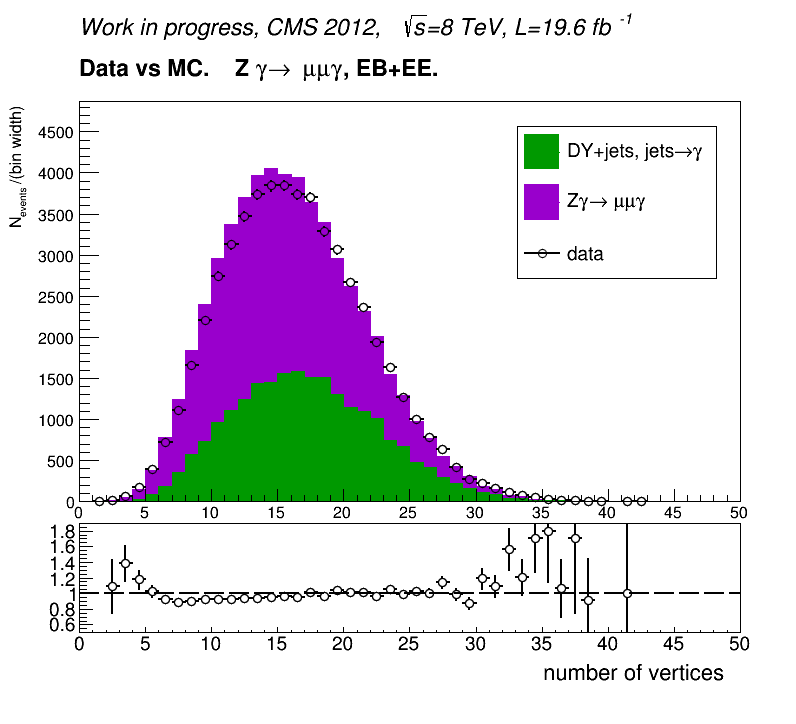
\includegraphics[width=0.45\textwidth]{../figs/figs_v11/MUON_ZGamma/PrepareYields/c_TotalDATAvsMC_EtaCommon__nVtx_noPU.png}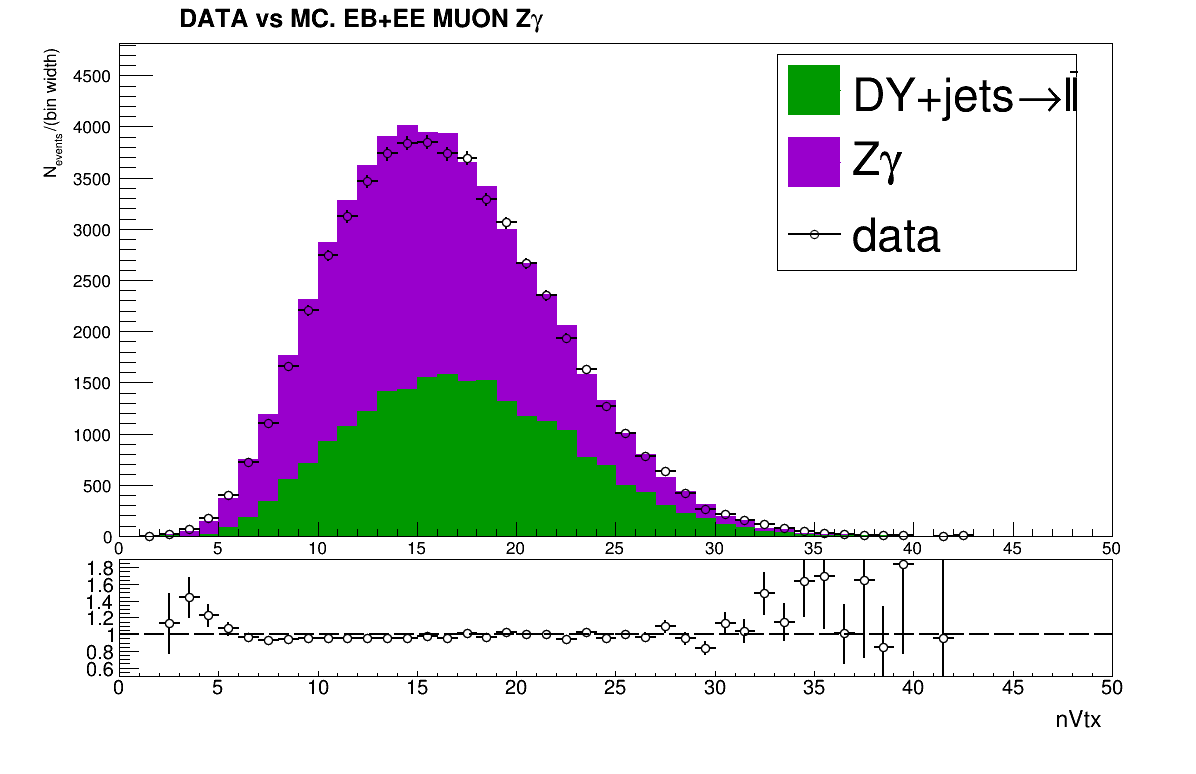
\includegraphics[width=0.45\textwidth]{../figs/figs_v11/MUON_ZGamma/PrepareYields/c_TotalDATAvsMC_EtaCommon__nVtx.png}
  \caption{Plots ofnumber of vertices, Data vs MC plots. $Z\gamma$ selected sample, muon channel. Left: no PU reweighting applied, right: PU reweighting applied. }
  \label{fig:DATAvsMC_nVtx}
  \end{center}
\end{figure}

Our $Wjets$, $DYjets$ and $t\bar{t}jets$ simulation samples partially contain $W\gamma$, $Z\gamma$, $t\bar{t}\gamma$ events. To remove the overlap, we did the following, relying totally on the generator-level (gen-level) information available in $Wjets$, $DYjets$, $t\bar{t}jets$ samples:
\begin{itemize}
  \item loop over all gen-level photons available in the sample;
  \item the event is removed from selected sample if at least one photon satisfy the following criteria:
  \begin{itemize}
     \item has $P_T^{\gamma}>10~GeV$;
     \item originates from lepton, boson or quark; and
     \item is separated by $\Delta R(\gamma,l)>0.4$ from at least one generated level muon or electron, depending on the channel.
  \end{itemize}
\end{itemize}
\noindent{A good data vs simulation agreement for the $Z\gamma$ plots in Fig.~\ref{fig:DATAvsMC_nVtx} validates the procedure.}

\subsection{Selected Events}

%Distributions of $P_T^{\gamma}$ and $M_T^W$ of the selected events are shown in Fig. \ref{fig:DATAvsMC} and \ref{fig:DATAvsMC_WMt}. 
%The is a large discrepancies in all the distributions and therefore the data-driven background estimates are necessary.\\

Distributions of $P_T^{\gamma}$ of the selected events are shown in Fig.~\ref{fig:DATAvsMC}. The is a large discrepancies in all the distributions and therefore the data-driven background estimates are necessary.

\begin{figure}[htb]
  \begin{center}
   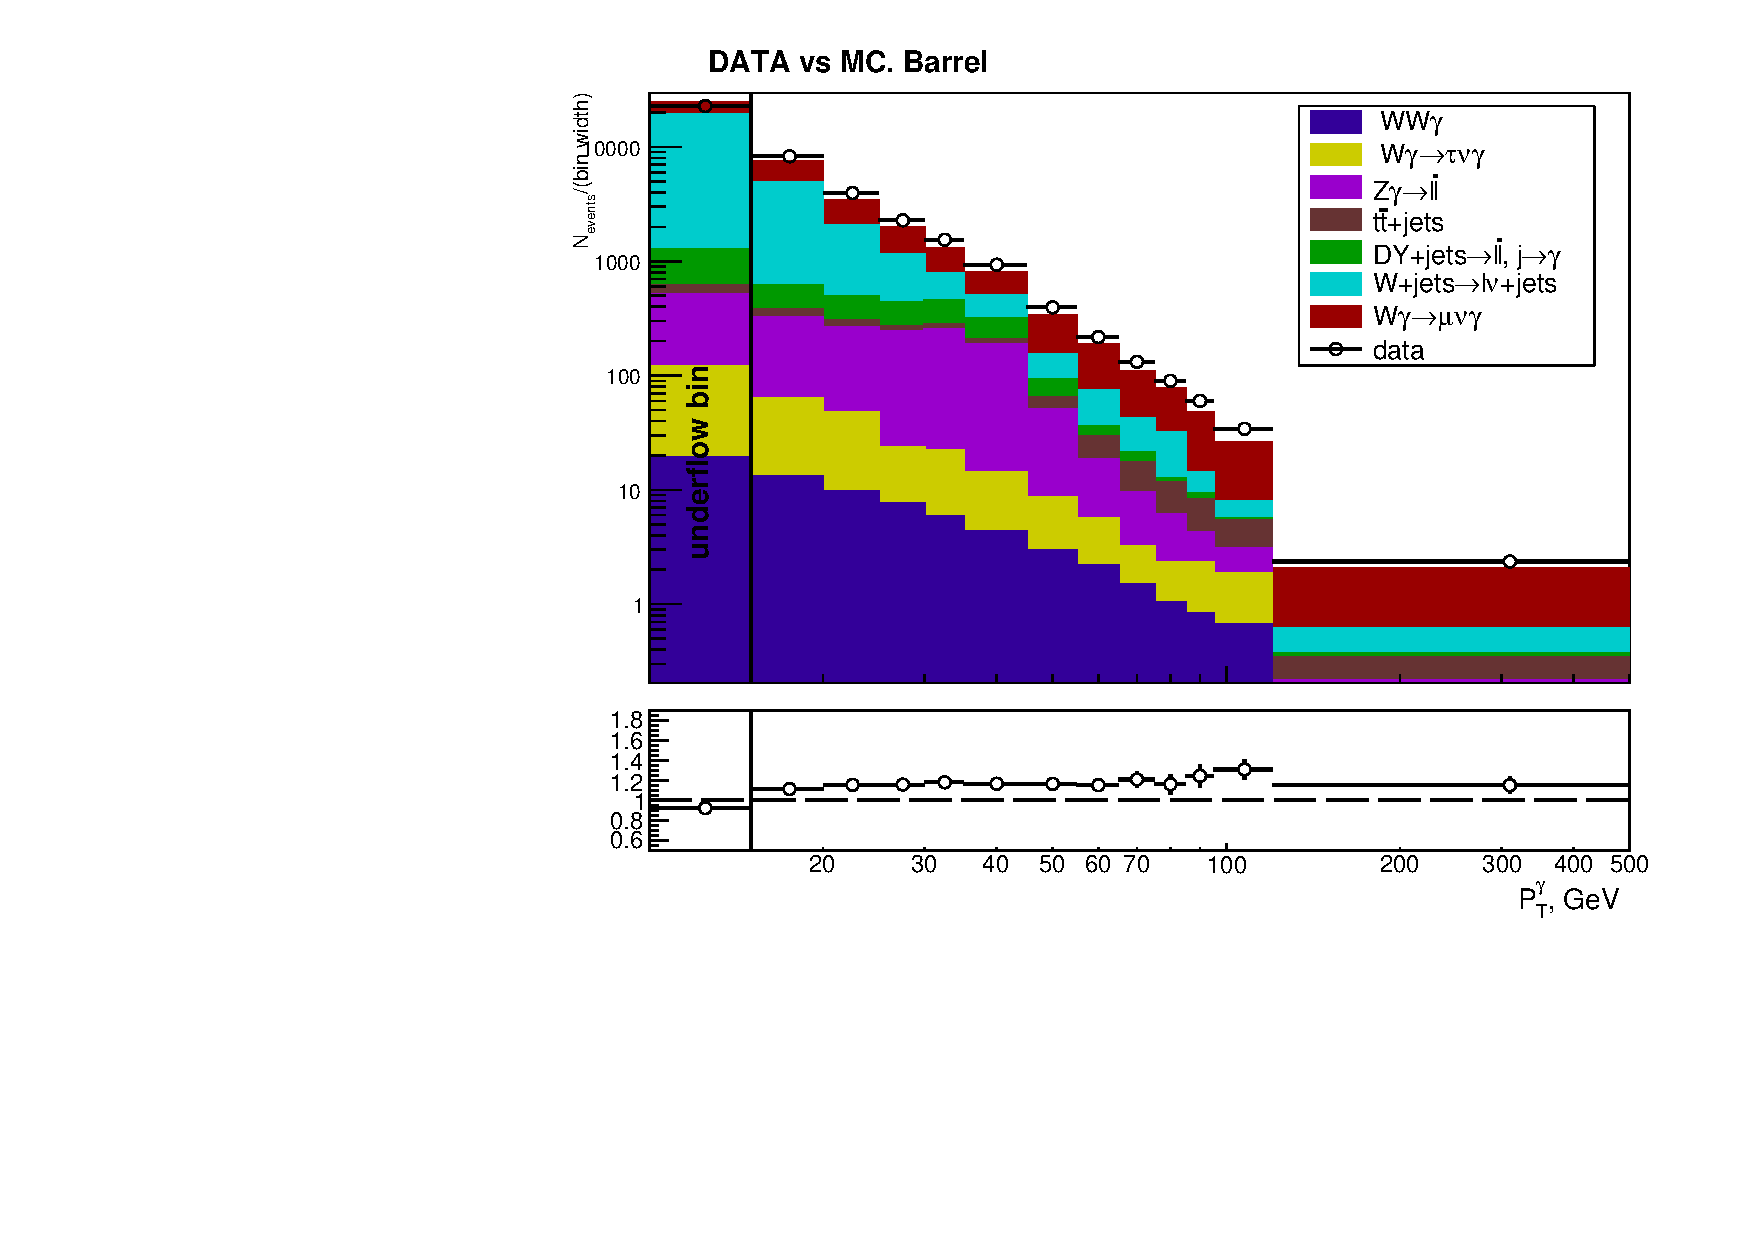
\includegraphics[width=0.45\textwidth]{../figs/figs_v11/MUON_WGamma/PrepareYields/c_TotalDATAvsMC_Barrel__phoEt.pdf}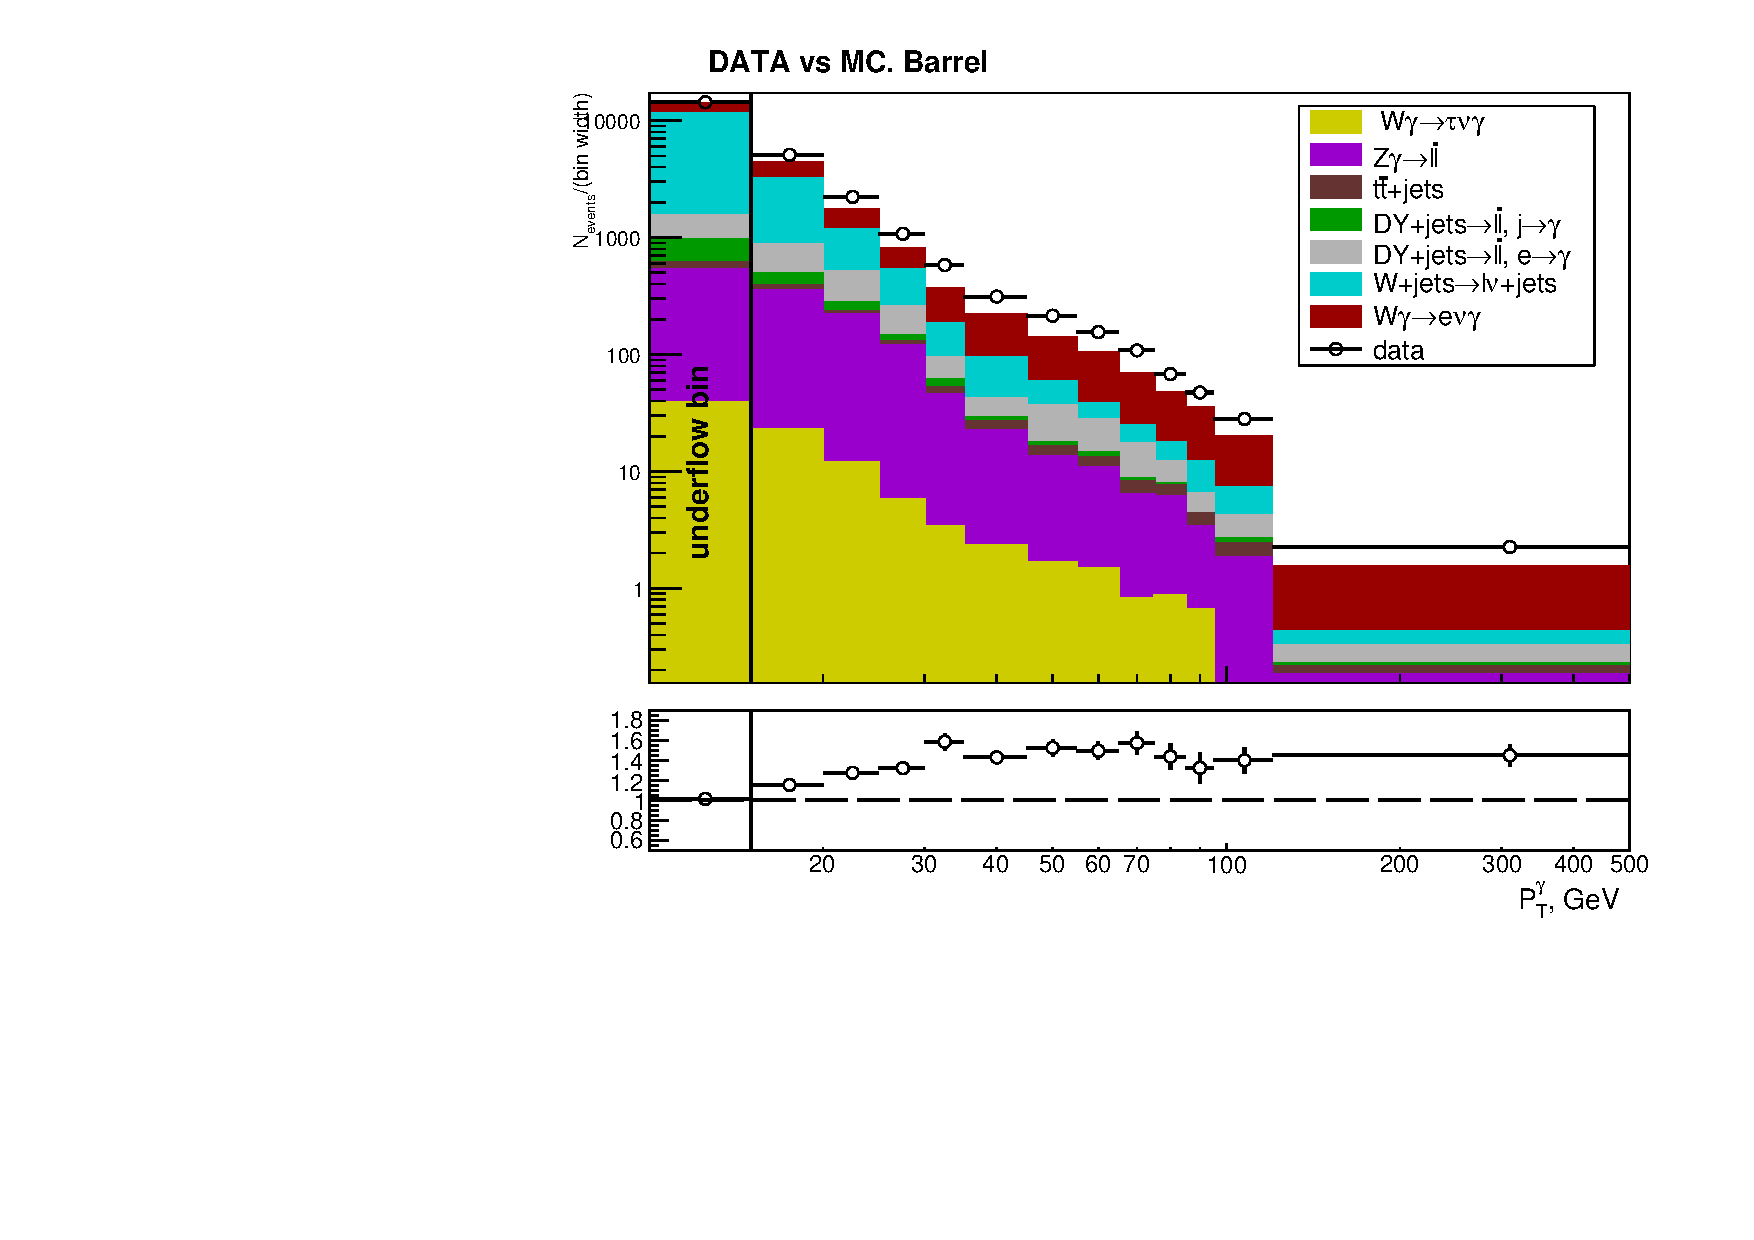
\includegraphics[width=0.45\textwidth]{../figs/figs_v11/ELECTRON_WGamma/PrepareYields/c_TotalDATAvsMC_Barrel__phoEt.pdf}
   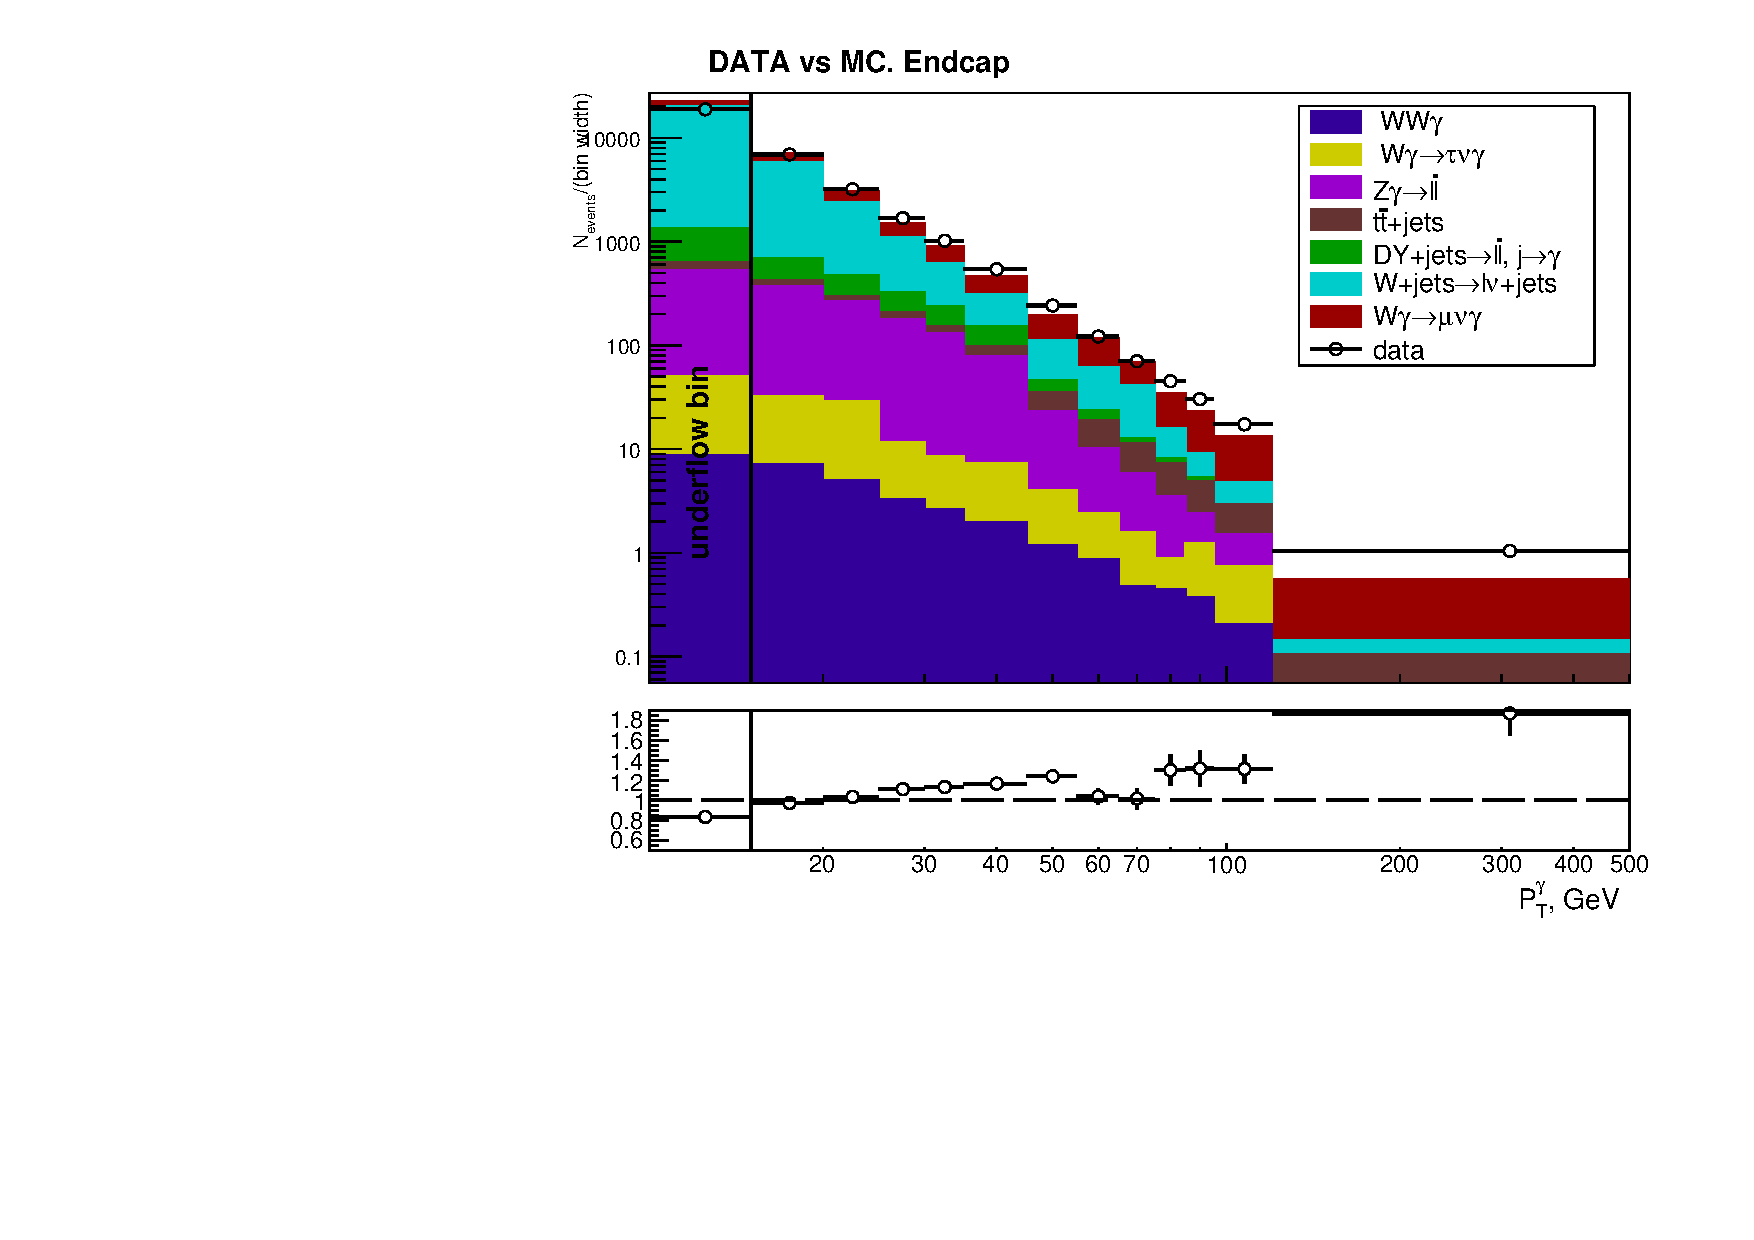
\includegraphics[width=0.45\textwidth]{../figs/figs_v11/MUON_WGamma/PrepareYields/c_TotalDATAvsMC_Endcap__phoEt.pdf}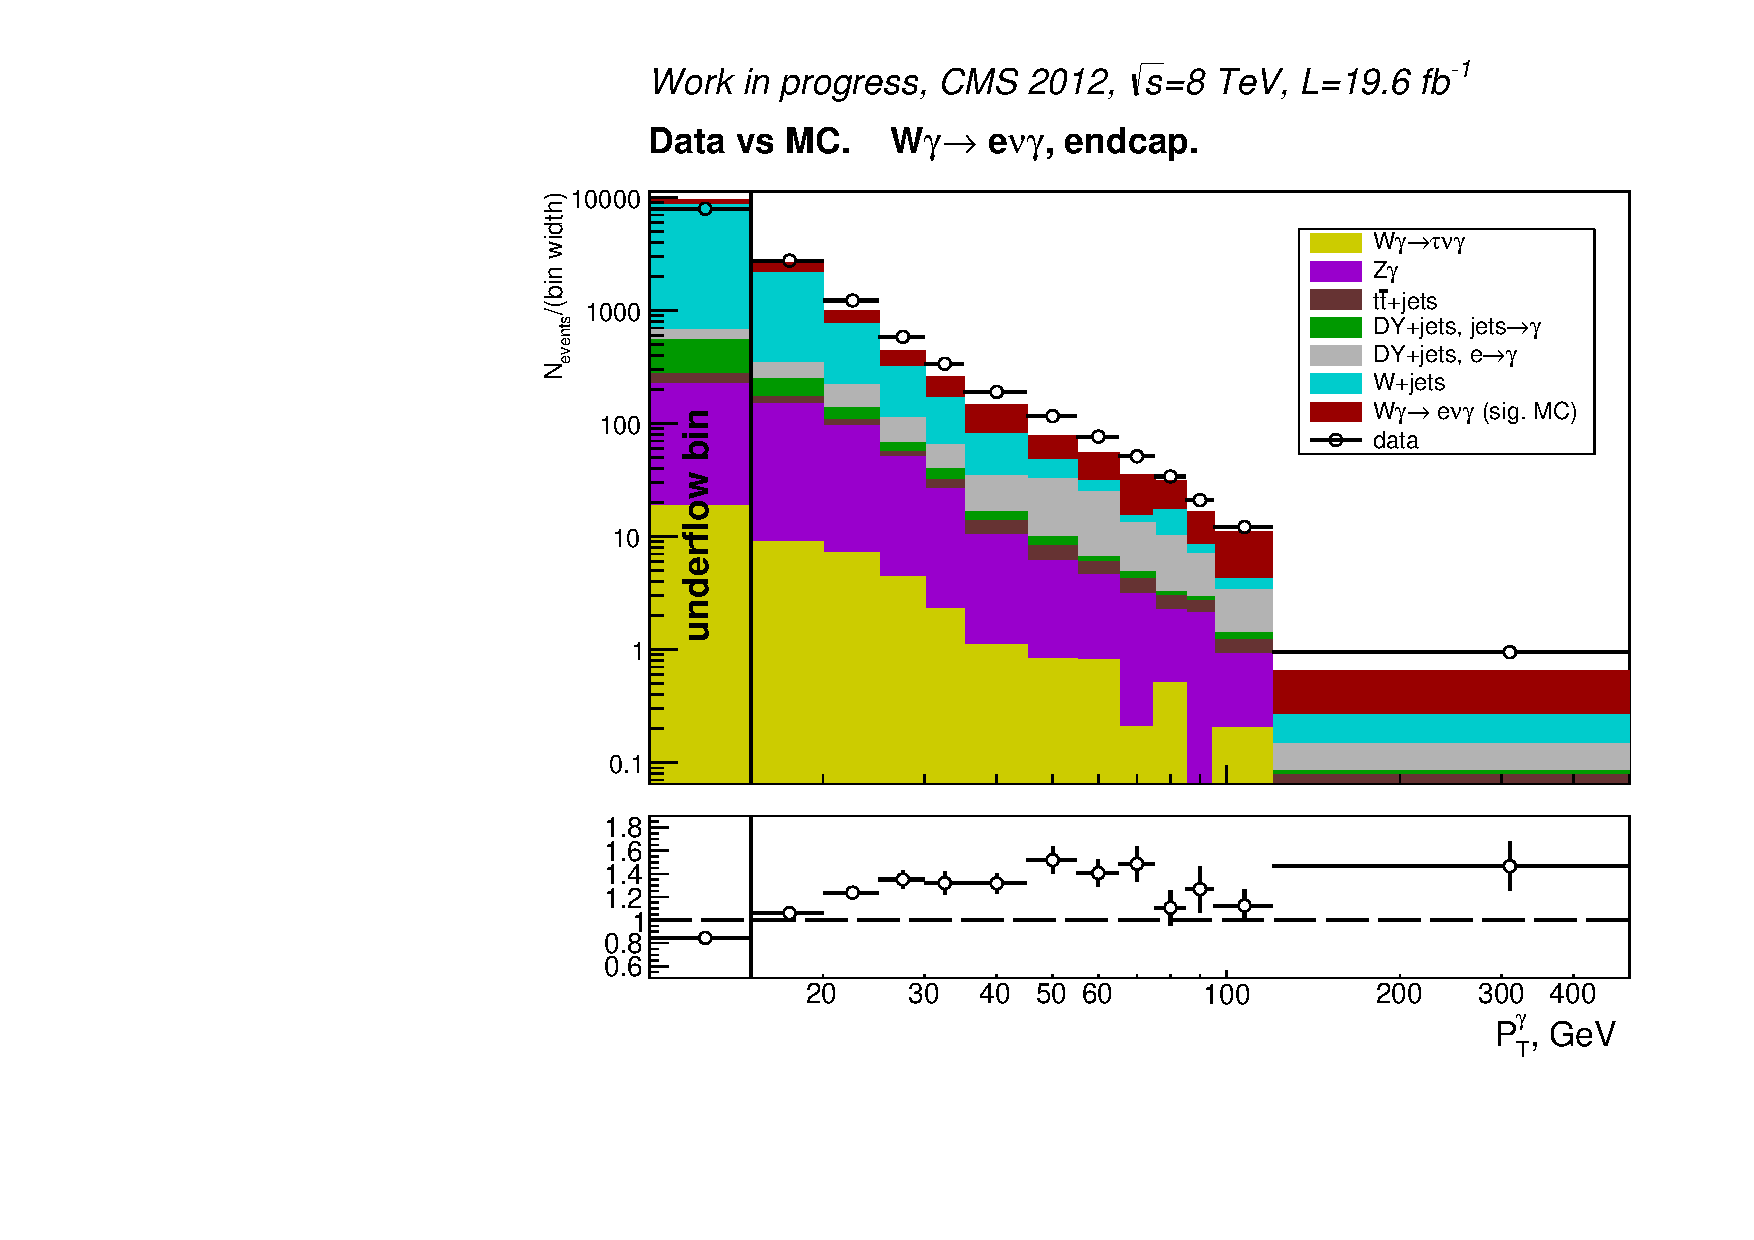
\includegraphics[width=0.45\textwidth]{../figs/figs_v11/ELECTRON_WGamma/PrepareYields/c_TotalDATAvsMC_Endcap__phoEt.pdf}
  \caption{Data vs simulation plots. Left column - muon channel, right column - electron. Top to bottom: barrel and endcap photons.}
  \label{fig:DATAvsMC}
  \end{center}
\end{figure}



%\begin{figure}[htb]
%  \begin{center}
%   \includegraphics[width=0.45\textwidth]{figs_v8/MUON_WGamma/PrepareYields/c_TotalDATAvsMC_Barrel__WMtVERY_PRELIMINARY.pdf}\includegraphics[width=0.45\textwidth]{figs_v8/ELECTRON_WGamma/PrepareYields/c_TotalDATAvsMC_Barrel__WMtVERY_PRELIMINARY.pdf}
%   \includegraphics[width=0.45\textwidth]{figs_v8/MUON_WGamma/PrepareYields/c_TotalDATAvsMC_Endcap__WMtVERY_PRELIMINARY.pdf}\includegraphics[width=0.45\textwidth]{figs_v8/ELECTRON_WGamma/PrepareYields/c_TotalDATAvsMC_Endcap__WMtVERY_PRELIMINARY.pdf}
%  \caption{Data vs MC plots, $M_T^W$. Left column - muon channel, right column - electron. Top to bottom: barrel and endcap photons. All selection criteria except $M_T^W$ cut on these plots. $15$~GeV$<P_T^{\gamma}<45$~GeV. The analysis cut of $M_T^W>40$~GeV is selected.}
%  \label{fig:DATAvsMC_WMt}
%  \end{center}
%\end{figure}
